\newcommand{\bmhHeroesFighterHeadline}{Krieger}
\newcommand{\bmhHeroesFighterToc}{Krieger}
\newcommand{\bmhHeroesFighter}{%

	\vspace*{1em}
	{

		\centering
\includegraphics[width=0.5\columnwidth]{\image{bmh/portrait_fighter.pdf}}

	}
	\vspace*{1em}

	\noindent
	Die Aufgabe des \keyword[Krieger]{Kriegers} ist es, an vorderster Front zu stehen und die Heldengruppe gegen die Kreaturen der Finsternis zu verteidigen. \say{Angriff ist die beste Verteidigung} ist dabei die Devise, egal mit welcher Waffe.

	Krieger der 1. Stufe sind mit einem Schwert bewaffnet und haben die besondere Fertigkeit \say{Rundumschlag} erlernt.

	\vfill

	{

		\centering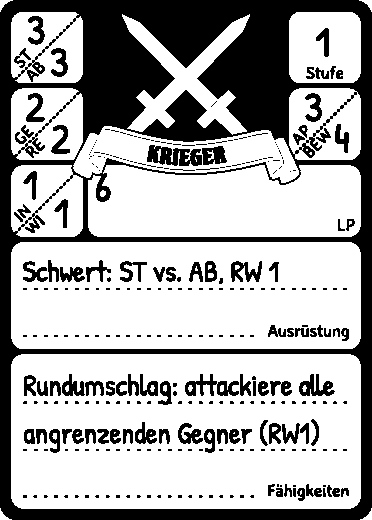
\includegraphics[angle=1,width=0.95\columnwidth]{\image{bmh/fighter.pdf}}

	}

	\columnbreak

	\noindent
	Die folgenden besonderen Fähigkeiten kann ein Krieger im Laufe seiner Karriere erlernen (siehe \refPage{lXP}).

	\medskip

	\power{Einzelkämpfer}{0 AP}{
		Du darfst mit einer \say{ST vs. ??} Waffe mit einem Zusatzwürfel angreifen, solange keine befreundete Kreatur näher als 4 Felder steht.
	}

	\power{Glück}{0 AP}{
		Du darfst eine deiner Proben neu würfeln und das für dich bessere Resultat zählt.
	}

	\power{Kraftreserve}{1 AP}{
		Du bekommst sofort 1 LP zurück.
	}

	\power{Kampftaktik}{1 AP}{
		Bis zum Ende deiner nächsten Runde können Kreaturen keine Gegenangriffe gegen dich ausführen.
	}

	\power{Rammbock}{0 AP}{
		Du bekommst beim Stoßen und Bugsieren einen Extrawürfel.
	}

	\power{Rundumschlag}{3 AP}{
		Attackiere alle Gegner in Reichweite 1 mit einer \say{ST vs. ??} Waffe.
	}

	\power{Schildkampf}{1 AP}{
		Bis zum Ende deines nächsten Zuges erhalten alle angrenzenden, befreundeten Kreaturen AB+1, solange du einen Schild führst.
	}

}

\newcommand{\bmhHeroesRangerHeadline}{Schütze}
\newcommand{\bmhHeroesRangerToc}{Schütze}
\newcommand{\bmhHeroesRanger}{%

	\vspace*{1em}
	{

		\centering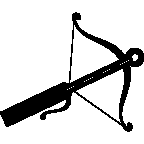
\includegraphics[width=0.5\columnwidth]{\image{bmh/portrait_ranger.pdf}}

	}
	\vspace*{1em}

	\noindent
	Der \keyword{Schütze} kann mit Fernkampfwaffen effektiv kämpfen, sollte sich jedoch nicht zu nahe an die Gegner heran trauen.

	Schützen der 1. Stufe sind mit einer Armbrust bewaffnet und haben die besondere Fertigkeit \say{Doppelschuss} erlernt.

	\vfill

	{

		\centering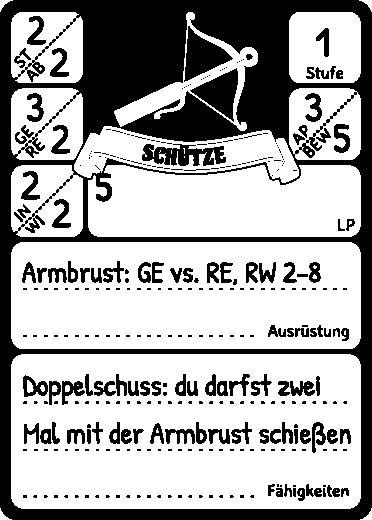
\includegraphics[angle=1,width=0.95\columnwidth]{\image{bmh/ranger.pdf}}

	}

	\columnbreak

	\noindent
	Die folgenden besonderen Fähigkeiten kann ein Schütze im Laufe seiner Karriere erlernen (siehe \refPage{lXP}).

	\medskip

	\power{Doppelschuss}{3 AP}{
		Du darfst zwei Mal mit einer Armbrust oder einem Bogen schießen.
	}

	\power{Glück}{0 AP}{
		Du darfst eine deiner Proben neu würfeln und das für dich bessere Resultat zählt.
	}

	\power{Lähmender Schuss}{2 AP}{
		Schieße mit einer Armbrust oder einem Bogen. Machst du mindestens 1 Schaden, ist dein Ziel auch [träge].
	}

	\power{Gezielter Schuss}{2 AP}{
		Attackiere mit einer Armbrust oder einem Bogen. Machst du mindestens 1 Schaden, ist dein Ziel auch [schwach].
	}

	\power{Stellungswechsel}{2 AP}{
		Schieße mit einer Armbrust oder einem Bogen. Vor oder nach dem Schuss darfst du dich für 1 BEW bewegen, ohne dass du Gegenangriffen ausgesetzt bist.
	}

	\power{Verdrängungs-Schuss}{3 AP}{
		Schieße mit einer Armbrust oder einem Bogen. Für jeden Punkt LP, den dein Gegner verliert, erhälst du 1 BEW, mit dem du ihn bugsieren darfst, solange seine Distanz zu dir nicht geringer wird.
	}

	\power{Zielsicherheit}{3 AP}{
		Schieße mit einer Armbrust oder einem Bogen. Dein Gegner erhält keine Bonuswürfel durch eingeschränkte Sicht. Außerdem darfst du die Nachteile von düsterem Licht ignorieren.
	}

}

\newcommand{\bmhHeroesThiefHeadline}{Schurke}
\newcommand{\bmhHeroesThiefToc}{Schurke}
\newcommand{\bmhHeroesThief}{%

	\vspace*{1em}
	{

		\centering
\includegraphics[width=0.5\columnwidth]{\image{bmh/portrait_thief.pdf}}

	}
	\vspace*{1em}

	\noindent
	Der \keyword{Schurke} unterstützt die Gruppe mit seinen zahlreichen Talenten und kümmert sich gern um Fallen oder geheime Wege. Im Kampf zieht er es vor, aus dem Hinterhalt zuzuschlagen und zu verschwinden, ehe die Gefahr zu groß wird.

	Schurken der 1. Stufe sind mit einem Dolch bewaffnet und haben die besondere Fertigkeit \say{Hinterhalt} erlernt.

	\vfill

	{

		\centering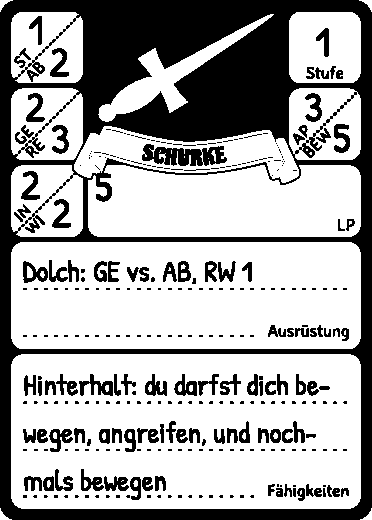
\includegraphics[angle=-1,width=0.95\columnwidth]{\image{bmh/thief.pdf}}

	}

	\columnbreak

	\noindent
	Die folgenden besonderen Fähigkeiten kann ein Schurke im Laufe seiner Karriere erlernen (siehe \refPage{lXP}).

	\power{Fallenspezialist}{2 AP}{
		Du kannst eine an dein Feld angrenzende Falle automatisch entschärfen.
	}

	\power{Flinke Finger}{0 AP}{
		Gegenstände aufzuheben oder abzulegen kosten dich 0 BEW und du kannst dies jederzeit auch ohne Bewegungs-Aktion tun.
	}

	\power{Glück}{0 AP}{
		Du darfst eine deiner Proben neu würfeln und das für dich bessere Resultat zählt.
	}

	\power{Hinterhalt}{3 AP}{
		Du darfst dich bewegen, angreifen, und nochmals bewegen.
	}

	\power{Läufer}{0 AP}{
		Deine BEW-Wert steigt permanent um 1.
	}

	\power{Sand in die Augen}{3 AP}{
		Attackiere mit \say{GE vs. ??}. Machst du Schaden, wird dein Ziel nicht verletzt, ist aber bist zum Ende deiner nächsten Runde [blind].
	}

	\power{Spürnase}{0 AP}{
		Beim Suchen darfst du einen Extrawürfel werfen.
	}

}

\newcommand{\bmhHeroesClericHeadline}{Kleriker}
\newcommand{\bmhHeroesClericToc}{Kleriker}
\newcommand{\bmhHeroesCleric}{%

	\vspace*{1em}
	{

		\centering
\includegraphics[width=0.5\columnwidth]{\image{bmh/portrait_cleric.pdf}}

	}
	\vspace*{1em}

	\noindent
	Der \keyword{Kleriker} zieht in die Schlacht, um das Übel der Welt zu richten. Außerdem heilt und stärkt er die Kräfte seiner Mitstreiter im Namen seiner Gottheit.

	Kleriker der 1. Stufe sind mit einem Steitkolben bewaffnet und haben die besondere Fertigkeit \say{Heilgebet} erlernt.

	\vfill

	{

		\centering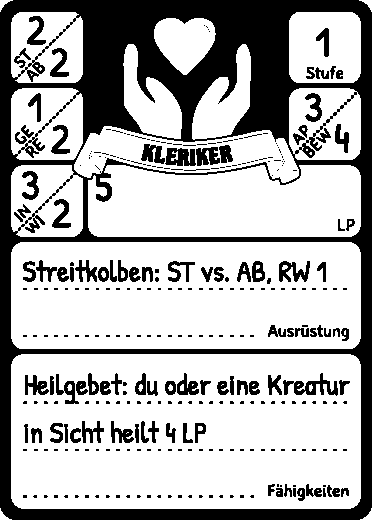
\includegraphics[angle=-1.25,width=0.95\columnwidth]{\image{bmh/cleric.pdf}}

	}

	\columnbreak

	\noindent
	Die folgenden besonderen Fähigkeiten kann ein Kleriker im Laufe seiner Karriere erlernen (siehe \refPage{lXP}).

	\power{Aura der Gerechten}{2 AP}{
		Bis zum Ende deiner nächsten Runde muss jede feindliche Kreatur, die am Zug ist, sich erst so lange Bewegen, bis sie mindestens 4 Felder Distanz zu dir zu erlangt hat.
	}

	\power{Einsicht}{1 AP}{
		Du darfst den SL darum bitten, auf der Battlemap alles einzuzeichnen, das sich hinter einer geschlossenen Türe befindet. Aufgedeckte Kreaturen dürfen nicht ziehen, ehe sie Sicht zu euch bekommen.
	}

	\power{Glück}{0 AP}{
		Du darfst eine deiner Proben neu würfeln und das für dich bessere Resultat zählt.
	}

	\power{Göttlicher Beistand}{3 AP}{
		Du und alle befreundeten Kreaturen am Spielplan heilen 1 LP.
	}

	\power{Hand auflegen}{2 AP}{
		Du oder eine benachbarte Kreatur deiner Wahl heilt 4 LP.
	}

	\power{Reinigendes Gebet}{2 AP}{
		Du oder eine befreundete Kreatur in Sicht darf bis zu zwei Zustände ihrer Wahl streichen.
	}

	\power{Verdammnis}{3 AP}{
		Eine befeindete Kreatur in Sicht wird [verflucht].
	}

}

\newcommand{\bmhHeroesWizardHeadline}{Magier}
\newcommand{\bmhHeroesWizardToc}{Magier}
\newcommand{\bmhHeroesWizard}{%

	\vspace*{1em}
	{

		\centering
\includegraphics[width=0.5\columnwidth]{\image{bmh/portrait_wizard.pdf}}

	}
	\vspace*{1em}

	\noindent
	Der \keyword{Magier} hat viel Zeit mit dem Studium alter Schriften verbracht, die ihn arkane Kräfte entfesseln und kontrollieren lassen, die Gegnern Schaden und Freunden helfen.

	Magier der 1. Stufe sind mit einem Zauberstab bewaffnet und haben die besondere Fertigkeit \say{Magischer Schild} erlernt.

	\vfill

	{

		\centering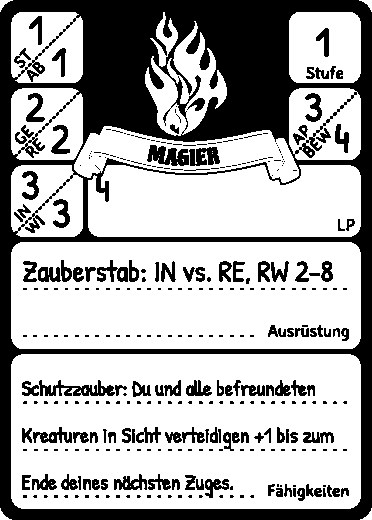
\includegraphics[angle=1.02,width=0.95\columnwidth]{\image{bmh/wizard.pdf}}

	}

	\columnbreak

	\noindent
	Die folgenden besonderen Fähigkeiten kann ein Magier im Laufe seiner Karriere erlernen (siehe \refPage{lXP}).

	\power{Barriere}{2 AP}{
		Zwei an einander angrenzende Kanten deiner Wahl innerhalb 1--8 Feldern werden bis zum Ende deines nächsten Zuges unpassierbar.
	}

	\power{Feuerball}{3 AP}{
		Nenne ein Feld in Reichweite 8, zu dem du zumindest eingeschränkte Sicht hast. Dort explodiert ein Feuerball. Du musst alle Kreaturen in dem Feld und in Reichweite 1--2 davon mit \say{IN vs. RE} angreifen.
	}

	\power{Glück}{0 AP}{
		Du darfst eine deiner Proben neu würfeln und das für dich bessere Resultat zählt.
	}

	\power{Magisches Geschoß}{2 AP}{
		Ein magischer Pfeil erreicht ungehindert von Wänden, Türen oder Kreaturen ein Ziel in Reichweite 1--6. Attackiere es mit \say{IN vs. AB}.
	}

	\power{Netz}{2 AP}{
		Ein klebriges Spinnennetz erscheint auf 10 zusammenhängenden Feldern deiner Wahl, eines muss an dich angrenzend sein. Die Felder werden zu schwierigem Gelände mit je 1 LP.
	}

	\power{Schutzzauber}{3 AP}{
		Du oder eine Kreatur in Sicht ignoriert bis zum Ende deine nächsten Runde den ersten Punkt LP-Verlust bei jedem Treffer.
	}

	\power{Teleport}{3 AP}{
		Du oder eine benachbarte, befreundete Kreatur darf von dir auf ein beliebiges, aufgedecktes Feld versetzt werden.
	}

}
